\section{\textbf{Methods}}

% how did I solve the problem?

% FUNDAMENTALLY, doing synthesis on the shipping, with a set of simple rules to validate observations.
%shipping as sensor network -- a synthesis.

\subsection{Volunteered ship information}

%"In short, changing technology and economics are moving map production from a system of unified central production to a local patchwork, and the old radial system of dissemination is being replaced with a complex network."
% -- Goodchild cartography paper, old and captures the change in production that is ongoing.

%\citep{elwood2011researching} includes refernce to these same layers, capturing data on 'core' data layers independently. Covers much of what Goodchild has discussed in terms of issues with VGI and its current 'cutting edge'
Historically, ship data was collected both by governments for internal use, and by private corporations with the intent to sell. As elsewhere in the production of geographic facts, a shift is underway which moves the emphasis away from top-down primary data collection, to instead relying on observations from a multitude \citep{goodchild1999cartographic,goodchild2007citizens,elwood2011researching}. Because of the limited authorative ocean information available, this has the potential to fundamentally change our use of the ocean.

% Using two kinds of volunteered ship data - needs to be handled in special ways:
% describe VOSclim data:
Ship captains have always taken climate observations alongside known location. % XXX CITE: old climate? what else? for what reason? 'since XXX, '.
Building on this history, the Voluntary Observing Ship (VOS) \citep{VOSOverview} program has collected a dataset spanning over 20 years and covering 10\textendash20\% of commercial traffic within each year. The primary purpose of the data is to collect open-ocean climate observations, so many of the records lack ship attribute information, making trajectory reconstruction difficult. The data is contained within the greater International Comprehensive Ocean-Atmosphere Data Set (ICOADS) dataset, and though the data is both spatially and statistically biased \citep{Wang2007}, it still can serve as a useful 'training' dataset on ship movements in the open ocean. Here, we use VOS records from 2003--2011, a dataset of 68.8 % XXX FIX THIS NUMBER
million records to provide validation and cross reference the rest of our observations.

% describe AIS data
The Automatic Identification System (AIS) \citep{Tetreault2002} was developed to improve maritime safety and prevent collisions by providing mariners local situational awareness. By locating the ships via global positioning satellite (GPS) signal, and broadcasting the location and other attributes (Table \ref{table:ais-broadcast-attributes}) at regular intervals via VHF transceiver \citep{Itu-r2010}, ships get a real-time display of local ship traffic, invaluable in inclement weather or rescue operations.  The International Maritime Organization (IMO) mandates that all ships $\geq150$ gross tonnage (GT) or ships bearing passengers carry AIS units, which has lead to approximately 200,000 ships being outfitted with AIS equipment, including all tankers, cargo ships and passenger vessels. Because the original intent of the data was improving maritime safety, well-understood VHF radios were used, broadcasting out to about 40km between ships. Since then, land-based folks, including ports, maritime professionals and amateurs, have come to realize that by merely setting up VHF antennae, data on local ship traffic can be obtained at a range of up to 100km at little cost. This has led to a number of sites providing real-time feeds of ship movement, such as MarineTraffic.com \citep{MarineTraffic}, aggregating the records from many land-based antennae and displaying them over both the web and via Google Earth. 

For the purposes of this study, 14 months of data were collected, from November 2011--December 2012, aggregating records provided by the three major online AIS providers: FleetMon, VesselTracker, and MarineTraffic. All three providers have Keyhole Markup Language (KML \cite{KML}) files for their data, intended to be used for import into Google Earth. At ten minute intervals, I requested these KML files from each of the providers, and then parsed each of the observations within the dataset, normalized to handle encoding differences between the providers, and finally inserted it into a spatial database, (PostGIS, \cite{ramsey2005postgis}), an extension providing support for OGC simple features on top of the PostgreSQL \citep{postgresql} object-relational database engine). Doing this over a 14 month period built up a dataset of 2.37 billion ship observations, which include not just ship location and time, but also many attributes as detailed in (Table \ref{table:ais-broadcast-attributes}).

In addition to these two datasets of ship observations, a number of ancillary data was identified to provide validation against the raw observations. These include: 

\begin{enumerate}
  \item Vessel databases, a tabular listing of ships along with a number of attributes, both contained in AIS records and not otherwise available. Approximately 250,000 vessels are contained in this database.
  \item Port databases, containing coordinates and berth details for ports globally, approximately 5,000 ports were identified from a variety of volunteered and authoritative sources.
  \item A high resolution land-sea mask, here derived from SRTM Water Body Data (SWBD), which classifies the world into either land or sea at three arc seconds resolution $56\deg$ S to $60\deg$ N, a byproduct of the SRTM digital terrain project. Additional data was for the areas beyond these bounds.
  \item Approximate information on ship movement patterns, based on historical charts such as a CIA vessel movement chart from the cold war.
  \item The original ship model I produced as part of the previous modeling effort \citep{Halpern2008}.
\end{enumerate}
% XXX EXPAND THIS LIST: ITU, FCC, Vesseltracker, DigitalSeas: THIS SHOULD BE MULTIPLE PAGES LONG...

\subsection{Validating the data}

The raw observations are full of caveats: because of the protocol design, there is no direct way of validating an incoming packet. So, as seen in (Figure \ref{fig:ais-obs-nov-2011}), many locations clearly on land have observations present, including a particularly thick band centered around the prime meridian. These records are more likely due corruption of longitude coordinate than reverence of Greenwich. Alongside transmission errors are operator error: the attributes which are sent alongside the time and position information are input by the mariners, and they may introduce errors in entry, or fail to update the attributes which change over time, such as the DESTINATION field. Each individual observation within this dataset is highly suspect, and generally the data is best treated as 'guilty until proven innocent'.

While there are numerous problems with the data, the large volume of data, and the compiled ancillary datasets, provide options to use the data via cross-correlation, improving accuracy and minimizing the number of raw observations required to build a model representation of the data. Two areas relevant to this problem are geographic data mining \citep{miller2009geographic}, and the recent work of \citep{goodchildli2012}. Here, we borrow the framework described in the latter work, and explore three avenues of quality assurance: crowd sourcing, social, and geographic approaches.

\subsubsection{crowd-sourcing}
% based (large volume of obs, multiple sources. Crowdsourced ref material)
% XXX EXPAND EXPAND, talk about authority and what it means
While \citep{goodchildli2012} found that crowd-sourcing was generally inadequate for VGI, it can function when the domain is limited and the pool of expertise is vast (as in the case with much open source software). In one sense, crowd-sourcing comes into play in this data when multiple radio towers of differing quality and origin receive records, across a variety of sources. Cross-referencing these sources then provides a consistency, though this doesn't rely on many citizens cross-referencing, but rather validates across their equipment.

\subsubsection{social}
% XXX EXPAND LIKE A MOFO
Mariners do provide regular updates to the various online services as to their attributes, so the attribute data pulled from these sources tends to be high. The ship operators often have the best working knowledge ships' data, much like someone who lives in a specific neighborhood is likely to have a better understanding of local geography. The ship operators can then communicate the data up to various shipping related aggregation sites, who operate the higher levels of the hierarchy, and rely on a group of trusted users for vetting incoming updates.

\subsubsection{geographic}
% XXX this is BLEH right now, make it not crap.
This brings us to perhaps the most important validation technique: using geography to validate the records. In this case, the individual observations are time-stamped points which precludes complex rule-based geometry checks, but we can rely on a few simple sets of tests:

In addition to our point location $\langle x,t \rangle$, we have multiple attributes $\langle z \rangle$ attributes alongside it, proving us a spatio-temporal observation $\langle x,t,z \rangle$. By cross-referencing the attributes, we can get a sense of how likely the attribute-only component of the record is, and infer from that how likely we are to have a valid geometry and timestamp.

We can also impose some basic validation on the geometries by referencing other geographic facts, as is used in the most pedestrian of GIS functions, the overlay analysis. By checking the data against a land-sea mask, we can make estimations as to when the provided location is a physical impossibility. One trick to this is that many ships do travel by river, so these rules must be careful to define what is a traversable area. Additionally, shallow water bodies impose additional constraints on many ships with positive draft. This could be validated (showing for example, the large berth oil tankers keep from land), but hasn't been implemented here.

For many classes of vessels, ships move between ports. Ships which exhibit movement patterns inconsistent with this goal are suspect, though there are other 'nodes' in the ocean which require inclusion, such as ballast water exchange points, such as the one located 200km offshore of California (Figure \ref{fig:cal-cargo}), and canals, which provide a means of ships to move between otherwise inaccessible locations. However, this remains a powerful validation technique: because the high resolution data is clustered around the shores with strong coverage at the ports, we get a disproportionately good look at the vessels in transit between this constrained set of locations.

As in many large dataset, the distribution of observations per ship follows an approximate power-law distribution. Using the raw number of observations received in our 14 month window provides another filter. A peak in the kernel density estimation (Figure \ref{fig:obs-per-vessel-log}) is seen around $10^4$ observations, with a clear drop-off after $10^5$ which is consistent with the theoretical maximum (one observation in every sample) of about $6.8 \times 10^5$.

\begin{figure}[htbp]
  \centering
  \includegraphics[width=100mm]{figures/obs-per-vessel-log.pdf}
  \caption{Number of observations per vessel, log scaled.}
  \label{fig:obs-per-vessel-log}
\end{figure}


% highlight importance of geometry + ATTRIBUTES. one alone is insufficient, both can be powerful.

% - geographic filtering 
%   + PORTS
%   + LAND/SEA MASK
%   + ...
% Link above with Goodchild thoughts on VGI and quality.

%An aside on 'ships' - ships can have multiple callsigns, MMSI idenfiers, and other data which ideally would locate a specific vessel. We handle this ambiguity methods -- a full version of this can go into supplementals, but worth covering here, because we can map \textbf{type} from observed behavior -- fishing vs. cargo vs. cruise is all obious when looking at the movement patterns (fold into above 'filtering process' section)

Another important point is that while ships provide us some details as to their nature, the categories provided here (such as tanker or cargo) are not based purely on attributes, but also include movement patterns. This is a key distinguishing characteristic between the data, different classes of vessels show distinct movement patterns, which is useful both as validation, and as an output product, since different classes of vessels have different sets of effects and interactions. Because this data is stored in a spatial database, we can link any derived representation back to the records that formed it. While this is a common feature of spatial databases, its an important trait since generally scientists are provided a simple 'end product' without the provenance trail which backs the specific data being provided.

%Can link data representations all the way back to attributes of raw data [note: this is true in many spatial databases, right? what makes it special here?]
% - often a requirement but only get 'end products' instead without detailed attributes, or conversely all details on one ship but no way to move between realms fluidly.

% overview of summary statistics of data - intermadiate workflow product
\begin{table}[htbp]
  \begin{tabular}{rrrrll} %{\centering\arraybackslash}p{2cm}>{\centering\arraybackslash}p{5cm}>{\centering\arraybackslash}p{9cm}}
    \hline
    Type & Vessels & fleet size \textit{(data)} & fleet size \textit{(cited)} & coverage (\%) & observations (M) \\
    \hline
    Cargo & 58510 & 32970 & 33392\textsuperscript{1} & & 665.45 \\
    Pleasure & 71388 & 57617 & ~800,000\textsuperscript{2} & & 267.48 \\
    Support & 23496 & 21425 & 25234\textsuperscript{1} & & 298.02 \\
    Tanker & 19363 & 20503 & 14068\textsuperscript{1} & & 264.42 \\
    Passenger & 8296 & 7182 & 6370\textsuperscript{1} & & 142.16 \\
    Fishing & X & 28544 & 51200\textsuperscript{3} & & 6.87 \\
    Other & X & 29077 & -- & -- & 4.75 \\
    High-speed & 2434 & 1178 & 1454 & 0.81 & 2.52 \\
    Authority & X & 1308 & X & & 1.44 \\
  \end{tabular}
  \caption{Summary of analyzed ship data\\
  1. \cite{Equasis2011}.\\
  2. \cite{westwood2001global}.\\
  3. \cite{FAOfishing}.}
  \label{table:ships-by-type}
\end{table}
% XXX: high-speed craft from ISL? can't find original ref
% NOTE: the FAO estimates the _full_ fishing fleet size at 4 million vessels, the size clearly has an important effect.

% Equasis 'state of the fleet' report (2011):
% NOTE: also has a helpful list in annex I of what comprises each class.
%   container/cargo [total: 
%     general cargo: 17034
%     specialized cargo:  250
%     roro cargo: 1537
%     container ships: 4974
%     bulk carriers: 9597
%   tankers:
%     oil and chemical tankers: 11828
%     gas tankers: 1574
%     other tankers: 666
%   passenger ships: 6370
%   offshore vessels: 6692
%   service ships: 4442
%   tugs: 14110

% as listed in maritime economics 3e (2007): (all over 10,000 dwt only):
% http://books.google.com/books?id=PAi04qzmfucC&pg=PA69&dq=shipping+cargo+fleet&hl=en&sa=X&ei=Ei2YUOTaNs3oiwKhy4D4CA&ved=0CDYQ6AEwAA#v=onepage&q&f=false
% tankers: 8040
% bulk carriers: 14756
% general cargo: 25784
% specialized cargo: 6978
% total cargo: 47433
%   tugs: 11097
%   dredgers: 1612
%   cruise: 452
%   ferries: 3656
% total non-cargo: 26880
% total fleet size: 74398

% classes from joined clean.ships table:
% [NOTE: these may double count some ships].
% 'high-speed': 1178
% 'passenger': 7182
% 'cargo': 32970
% 'support': 21425
% 'authority': 1308
% 'fishing': 28544
% 'pleasure': 57617
% 'tanker': 20503
% 'other': 29077

% these came from our full obs table, but clearly have issues (such as: no fishing).
% high-speed: 2434
% cargo: 58510
% other: 0
% fishing: 0
% passenger: 8296
% pleasure: 71388
% support: 23496
% tanker: 19363
% authority: 0

\subsection{Data Representations}

% It is necessary to have multiple representations of the data - the data model must flow from the question asked (goodchild, also anything in ebook on GISci?)

After filtering and validating the data as described above, we want to begin building data representations which allow us to answer some of the questions highlighted in the introduction. As is the case in many datasets, there is no single optimal representation, but instead a set of representations which, when matched to particular uses, allows us to address interesting questions.

Here, we look at how maintaining both discrete object and continuous fields representations (Figure \ref{fig:representation-in-gis}) allow us to ask questions on shipping, including its ecological effects. The point data alone is insufficient for making predictions related to these phenomena, but neither can we incorporate too much complexity or we risk making computation infeasible and the data requirements beyond the scope of what we have at hand \citep{de2007geospatial}.

% Some of the effects. link up how specific effects could be monitored by our different repsentations. Can't just use points to predict phenomena of this nature, but can't incorporate full complexity of reality either; chosen representations are a compromise between those two extremes.

% As in \ref{fig:representation-in-gis}, we can keep track of the ships in a discrete object representation, and after filtering the observations, converting the individual ship locations into movement tracks.

% Merger of data - which can give a single representation of the data

\begin{figure}[htbp]
  \centering
  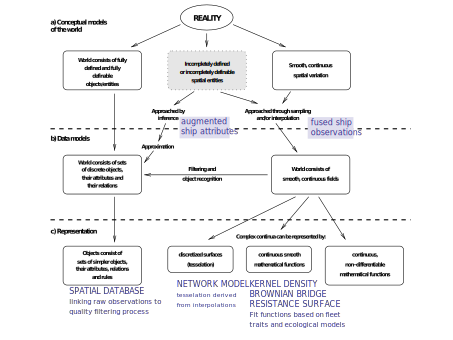
\includegraphics[width=160mm]{figures/representation-in-gis.pdf}
  \caption{GIS abstractions, this work's specific {\color{DBlue} additions in blue}. Adopted from \cite{Bivand2011}}
  \label{fig:representation-in-gis}
\end{figure}

% It is necessary to have multiple representations of the data - the data model must flow from the question asked (goodchild, also anything in ebook on GISci?)

%Want to link representation to USE, lack of a single simple view which meets all needs. counterpoint to the 'single metric' perspective. 
% [have note: 'link to stats', but now unsure what that means].

% Store the raw observations in a spatial database (PostGIS), use parallelized code to quickly aggregate the results.

\subsubsection{Raw point data}
 \begin{itemize}
   \item geoatom with time $\langle x,t,z \rangle$
   \item formalize what these observations mean
   \item apply filtering using space-time + attributes
 \end{itemize}

We have records sampled at 10 minute intervals (600 seconds). This is a reasonable approximation of paths for most of the observed movement patterns, and doesn't differ significantly from others who have aggregated to remove for noise (\cite{Vries2009}, which uses piecewise aggregate approximation with w = 30 (300 seconds) to 'strike a good balance between capturing the general movement and ignoring noise'. % NOTE: this is a filtering technique, so it isn't a direct mapping onto the reduced fidelity data we're using.

Spatial databases historical focus on accuracy \citep{goodchild1989accuracy}

\subsubsection{Tracks}
 \begin{itemize}
   \item link to time geography... Hagerstrands conceptual framework... Literature on T-GIS as tracking.
   \item Goodchild lecture on T-GIS mentioned track interpolation, inferences about activity, track convergence, etc

 \end{itemize}
 % [perhaps drop this for the time being... don't have lit built up on it, unless we can use the anomaly detection stuff]

\subsubsection{Field-based models}

Used kernel smoothing to produce these field-based estimates.

\paragraph{Density estimates of ships by type}

Why this matters: the view most people want to see; counts of X where and when. Useful for MSP, conflict resolution, detecting conflict zones, etc

\paragraph{Speed density estimations of ships by ship type}

Speed plays a critical role in determining the survivability of marine mammals from collisions (Vanderlaan, others), and speed also is the primary knob on the emissions profile of a particular vessel.

CLARIFY: what are the other effects of speed? anomaly detection?

\subsubsection{Network model of ship travel}

Some analyses require 'factoring out' geography to the extent possible, such as ecological models (Tilman book), Economic, et cetera. Network theory provides a useful basis of analysing geographically explicit data in a mathematical framework which can incorporate some of the geographic constraints while eliding many details necessary in a spatially-explicit model.

Best thing here is Kaluza but they totally lost the geography in transit -- can produce a middle ground model which has geographic nodes and edges, but still retains the rigour of the network model. Can get both!

% Paragraph from one of my position papers --
% One model I’m particularly interested in is hybridized network models using tools like NetworkX, which have the attractive property of allowing mixed field/object representations of the same data simultaneously, hence escaping the common limits of networks as mentioned in ? of every link or edge requiring a discrete value. By imbuing a network model with object-oriented features, some of the challenges I’ve been having representing my ship traffic data vanish. An- other advantage of manipulating graphs as a primitive is their widespread support, including general purpose graph databases which are particularly taking off in the semantic space.

% another pp from a position
% This becomes particular important as the tools of spatial thinking extend across disciplinary boundaries, both in the social and physical sciences (Goodchild and Janelle, 2010; Tilman and Kareiva, 1997). Other domains, such as ecology and economics, are coming to terms with the fact that their historical approaches to keeping simple models (and by extension, limiting model scope to their domain) ignores important spatial context which naturally arises at the unit of analysis (Tilman and Kareiva, 1997; Krugman, 1991).



% -----------------------------------------------------------------------------


% One advantage of linked data or hierarchical models is allowing cross-correlation among many datasets which may improve accuracy with less new measurement required. This is one appeal of volunteered geographic information: some uncertainty problems become tractable when we have orders of magnitude more observations , as we can evaluate the probabilistic distribution of a phenomena not by specifying a priori distributions, but instead allowing the large volume of samples to provide a distribution. Efforts to accomplish this include geographic data mining Miller and Han (2009).


% Volunteered Geographic Information (VGI) Goodchild (2007), involves participation of citizens in the production of georeferenced facts. Extending the ideas of User-generated content (UGC) to the specific nature of geographic information, a transition away from authority-based production means that information provided is often asserted rather than filtered through a formal quality control process. This shift requires new approaches to validate and quality-control VGI, while retaining its benefits in turnaround time and production cost. In Goodchild and Glennon (2010), a case study of disaster response is taken up, where real-time information is critical to save lives and minimize property damage, and the appeal of VGI is obvious.  

%\ldots

% Following up on Goodchild and Li (2012), three mechanisms for quality assurance are men- tioned: crowd-sourcing, social groups, and geographic. Hybridized approaches which use all three would be useful: rely on the size of the participation base to cross check (and improve sample size from a statistical perspective), use a social structure to defer in disputes and confer some of the virtues of authority, and use filtering which takes into account abstract geographic rules to impose constraints on the data.

% The approaches of machine learning and geographic data mining again seem particularly relevant here: as we build up cross referenced datasets on participants, we can infer much more despite the limits of each individual observation. In effect, this is what Currier et al. (2012) suggests, by adding information on who volunteers what, we can move toward solving the lingering semantic issues present in ’universal’ geographic information. One risk: much of the correlated information is controlled by a handful of organizations such as Google, Facebook and Twitter, which sell that information back to advertisers Lanier (2010) which limits the possibility of truly connected geographic facts, as the organizations have incentives to keep large parts of their information private.

\subsection{Record Linkage}

% XXX open problem: what designates a 'ship'?
%   Hal: `The biggest flaw is that, long ago, I assumed one ship == one callsign. It turns out, of course, that a single ship can have multiple callsigns (due to sale or reflagging), and that a single callsign can be assigned to multiple ships (e.g. NOAA, and also the Queen Mary/Queen Mary II). So the db really needs its own internal ship UID.`

%  Hal, on 'using MMSI + IMO + Callsign'--  Yeah, that still misses reflagging. I think what I will end up with is a "find-or-create ship with IMO,MMSI,Callsign", together with a manual process for me to force the database to combine two different ship UUID's that actually refer to the same ship. Even that isn't enough, because we see misprogrammed AIS units with dummy MMSI's, and fleetwide MMSI's."

%    ... Almost want a probabilistic model of what ship it is based on the information we do have reliably, and cross-validation with the various online databases... perhaps even validation with Equasis? Could do this for a small subset of the ships, but clearly not them all.

% TODO: perform data validation on these observations with Equasis. Sample a handful of records from each class, then perform the validation.

By combining authoratative data from a variety of sources (Table \ref{table:ships-data-sources}), we can reconcile our observations with known ship records, and greatly improve the quality of the resulting ship movement models. Though authoratative, the sources are also inconsistent, and require an initial step of cross-linking records, an approach commonly used in medical records [cite] and computer science [cite].

% table describing sources
% SOURCES: ship-id-model.txt
%          ship-id-model/linkages.txt
\begin{table}[htbp]
  \begin{tabular}{rrlll} %{\centering\arraybackslash}p{2cm}>{\centering\arraybackslash}p{5cm}>{\centering\arraybackslash}p{9cm}}
    \hline
    Source & abbr & records & cross-linked & attrs \\
    \hline
     Digital Seas & DS & 212166 & 68002 & name, imo, mmsi, callsign, type, width, length \\
     Federal Communications Commission: Universal Licensing System & FCC & 319964 & 24531 & name, mmsi, callsign, class, gross gonnage, length \\
     International Telecommunication Union: Maritime mobile Access and Retrieval System (MARS) & ITU & 372183 & 75928 & name, callsign, mmsi, class, owner, imo, gross tonnage\\ 
     VesselTracker & VT & 126534 & 83372 &  name, imo, mmsi, callsign, length, class, length
  \end{tabular}
  \caption{Ship data sources.}
  \label{table:ships-data-sources}
\end{table}

Here, we build a probabilistic model which evaluated all possible pairwise combinations between all source records. By using the methodologies of % XXX cite book, FRIL?
, we built a set of rules to map records between the six possible source pairs. Each pair was evaluated for attributes which had consistent data, and matched against these columns. The software used % XXX FRIL
provides an Expectation Maximization algorithm to iteratively optimize the weighting of columns, but due to the volume of data in our sources, this proved inefficient. Instead, samples of the data were examined, and the criteria were set by manual tuning both the weightings and acceptance levels to match a training dataset of valid linkages (Table \ref{table:ships-record-linkage-methods}. % XXX HUURR, write this better

For most fields, either the 'equal fields' (both fields are exactly the same) or the Jaro-Winkler distance metric were used. Jaro-Winkler has a useful properties for this data: it is effective on both numeric and textual data, and is particuarly useful in picking up the kinds of errors inherent in user-entered and sometimes poorly validated data sources such as those used in this study. A study of a variety of string comparison metrics \cite{Cohen2003} found it % XXX what?

CATCHING ERRORS:
 detecting errors in this data is particularly problematic because the records are highly correlated by nature -- similar imo, callsign and name for two different ships in the same fleet. have to keep those separate while linking small diferences due to entry error.

 wrote validate-ds-vt.py which encapsulates a bunch of useful rules for the edge cases, and I've visually inspected the results. it does a good job of finding our other 'missing matches'.

% table describing the record linkage technique used for each data source
% SOURCE: record-linkage/FRIL/config/*.xml
\begin{table}[htbp]
  \begin{tabular}{rrrrrr} %{\centering\arraybackslash}p{2cm}>{\centering\arraybackslash}p{5cm}>{\centering\arraybackslash}p{9cm}}
    \hline
    Source $A$ & Source $B$ & acceptance level & column & distance metric & weight \\
    \hline
     DS & FCC & 95 & callsign & equal & 99 \\
        &     &    & name & Jaro-Winkler & 1 \\
     DS & ITU & 92 & callsign & Jaro-Winkler & 50 \\
        &     &    & MMSI & equal & 40 \\
        &     &    & name & Jaro-Winkler & 40 \\
     DS &  VT & 85 & callsign & Jaro-Winkler & 60 \\
        &     &    & IMO & Jaro-Winkler & 20 \\
        &     &    & name & Jaro-Winkler & 20 \\
    FCC & ITU & 85 & callsign & Jaro-Winkler & 95 \\
        &     &    & name & Jaro-Winkler & 5 \\
    FCC &  VT & 95 & callsign & Jaro-Winkler & 66 \\
        &     &    & name & Jaro-Winkler & 5 \\
        &     &    & MMSI & Jaro-Winkler & 24 \\
        &     &    & length & equal & 5 \\
     VT & ITU & 80 & callsign & Jaro-Winkler & 20 \\
        &     &    & MMSI & Edit Distance & 30 \\
        &     &    & name & Jaro-Winkler & 10 \\
        &     &    & IMO & Jaro-Winkler & 40 \\
  \end{tabular}
  \caption{Ship record linkage methods used. \\
    \textsuperscript{1} Jaro-Winkler distance used length $l = 4$ and scaling factor $p = 0.1$}
  \label{table:ships-record-linkage-methods}
\end{table}

After pairwise linkage, matched records (Table \ref{table:ships-record-linkage-results-summary}) were further cross-referenced, to account for the fact that the same ship often appears in many of our sources. The number of links per ship averaged 3.5 ($\mu = 3.49, \sigma = 0.828$, ) % XXX STATISTICALLY SIGNIFICANT? a bunch with just a few.

% XXX move this table to an appendix? doesn't really help tell the story.
% table describing # of records linked betwen each source
% SOURCE: ship-id-model/matches.ods
\begin{table}[htbp]
  \begin{tabular}{rrll} %{\centering\arraybackslash}p{2cm}>{\centering\arraybackslash}p{5cm}>{\centering\arraybackslash}p{9cm}}
    \hline
    Source $A$ & Source $B$ & matched records & \% possible matched \\
    \hline
     DS & FCC &  3481 & 50.35\textsuperscript{1} \\
     DS & ITU & 41380 & 30.73 \\
     DS &  VT & 72286 & 53.68 \\
    FCC & ITU & 27874 & 50.58\textsuperscript{1} \\
    FCC &  VT &  5282 & 53.23\textsuperscript{1} \\
     VT & ITU & 54727 & 43.25 \\
  \end{tabular}
  \caption{Ship record linkage results summary. \\
    1. FCC data is US only, \% possible is of US-only data from each source.}
  \label{table:ships-record-linkage-results-summary}
\end{table}



% XXX what follows is the math for the Jaro Winkler equations, worth mentioning as they describe the primary method used for linking our records together.

% good code-based illustration at: http://www.gettingcirrius.com/2011/01/calculating-similarity-part-2-jaccard.html
% XXX MOVE THIS TO AN APPENDIX??
The Jaro distance:
\begin{equation}
  d_j = \left\{
  \begin{array}{l l}
    0 & \text{if }m = 0 \\ 
    \frac{1}{3}\left(\frac{m}{|s_1|} + \frac{m}{|s_2|} + \frac{m-t}{m}\right) & \text{otherwise} \end{array} \right.
\end{equation}

$ d_j $ Jaro Distance
m = number of matching patterns
t = number of transposed characters
|s1| = length of first string
|s2| = length of second string

\begin{equation}
  \left\lfloor\frac{\max(|s_1|,|s_2|)}{2}\right\rfloor-1
\end{equation}
range = max(length(a), length(b)) / 2 - 1


Jaro-Winkler distance:

\begin{equation}
  d_w = d_j + (\ell p (1 - d_j))
\end{equation}


